\documentclass{article}

\usepackage{../preamble}
\standalonetrue

\pagestyle{fancy}
\fancyhf{}
\rhead{Section \thesection}
\lhead{PHYS 304 Lecture 4}
\rfoot{Page \thepage}


\title{PHYS 304 Lecture 4}
\author{Ashtan Mistal}
\date{!!!}

\begin{document}

\ifstandalone
\maketitle
\fi

\graphicspath{{./Lecture04/}}

\section{Key points from last day}

Everything is a particle and a wave, where the particle-like behaviour is manifest when many purely harmonic waves with different wavelengths happen to add up to yield a more-or-less localized wavepacket (the particle).  

The recipe for finding the expectation value of any observable quantity that classically depends on $x$ and $p$ as $Q(x,p)$, is to replace $p$ in that function with the "operator" $-i \hbar \frac{\partial}{\partial x}$ and then use the following operator formula:

$$\langle Q(x,p) \rangle = \int \Psi^* \left[ Q(x, -i \hbar \frac{\partial}{\partial x} \right] \Psi dx$$

\begin{itemize}
    \item Keep in mind: What do we mean by "localization of wavelengths"?
    \item Note that the operator has to appear \textbf{after} $\Psi^*$ and \textbf{before} $\Psi$
\end{itemize} 


\section{Solving the Schrodinger Equation}

\subsection{Activity 1}

What is the time-independent Schrodinger equation?

$$- \frac{\hbar^2}{2m} \frac{\partial^2 \psi}{\partial x^2} + V \psi = E \psi$$

What is the space-independent Schrodinger equation?

$$\frac{d \phi}{dt} = - \frac{i E}{\hbar} \phi$$

How are these two equations related?

The full schrodinger equation:

$$i \hbar \frac{\partial \Psi}{\partial t} = - \frac{\hbar^2}{2m} \frac{\partial^2 \Psi}{\partial x^2} + V \Psi $$

What is the technique used to go about simplifying the solution to this second order partial differential equation?

We need to postulate a solution that is a product of time and space independent functions, then derive two partial differential equations that are simpler to solve, and intimately connected to one another. 

We call the constant that these two must be equal to $E$, hence relating the two. 


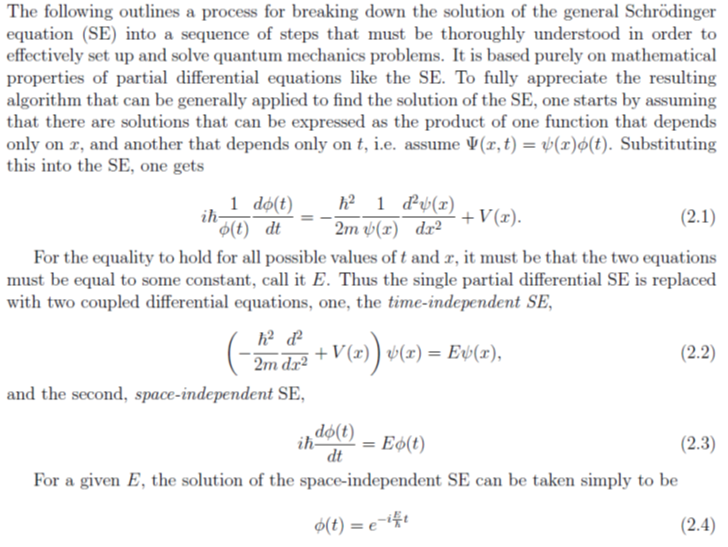
\includegraphics[width = 0.8 \textwidth]{Lecture04/1.png}

\subsection{Activity 2}

\begin{enumerate}
    \item Are there any restrictions on the solutions of the space-independent Schrodinger equation? (i.e. can it be solved for any value of $E$?)
    
    $$i \hbar \frac{d \phi(t)}{dt} = E \phi(t)$$
    
    And therefore $\Phi(t) = e^{-i \frac{E}{\hbar} t}$ for any real value of $E$. Imaginary values of $E$ would lead to un-normalizable wavefunctions. 
    
    \item Are there any restrictions on the solutions of the time-independent Schrodinger equation? (i.e. can it be solved for any real value of $E$?)
    
    $$\left( - \frac{\hbar^2}{2m} \frac{d^2}{dx^2} + V(x) \right) \psi(x) = E \psi(x)$$
    
    Although it isn't immediately obvious, we will see that depending on the potential profile, $V(x)$, there are typically only solutions of the time-independent SE for restricted values of $E = E_n$. Let us refer to the solution of the time-independent SE for a given value of $E_n$, as $\psi_n(x)$. Then, we know that the set of states $\Psi_n(x,t) = \psi_n(x) \phi_n(t) = \psi_n(x) e^{-i \frac{E}{\hbar} t}$ are all, separately, solutions for the full Schrodinger equation. Each such solution for a specific value of $E_n$ is called a \textit{stationary state}.
\end{enumerate}

\subsection{Activity 3, 4, and 5}

Why is $\Psi_n(x,t) = \psi_n(x) \phi_n(t)$, corresponding to a specific value of $E_n$, called a \textit{stationary state}? \textit{hint: find the expectation value of any operator $\hat{Q} (\hat x , \hat p)$ in an arbitrary stationary state.}

The expectation value is given by the following:

$$\langle Q \rangle (t) = \int_{- \infty}^\infty \psi^*_n(x) e^{-i \frac{E}{\hbar} t } \hat Q (\hat x, \hat p) \psi_n(x) e^{-i \frac{E}{\hbar} t } dx$$

Next, derive the expectation value of the energy when the particle is in a stationary state corresponding to a value $E_n$. 


Another interesting property of the stationary states is revealed by evaluating the expectation value of the total energy of the particle in an arbitrary stationary state:

$$\langle E \rangle (t) = \int_{- \infty}^\infty \psi^*_n(x) \left( - \frac{\hbar^2}{2m} \frac{d^2}{dx^2} + V(x) \right) \psi_n(x) dx$$


Derive the expectation value of the energy squared when the particle is in a stationary state corresponding to a value $E_n$.  What does this tell you about the variance of the measured energy?


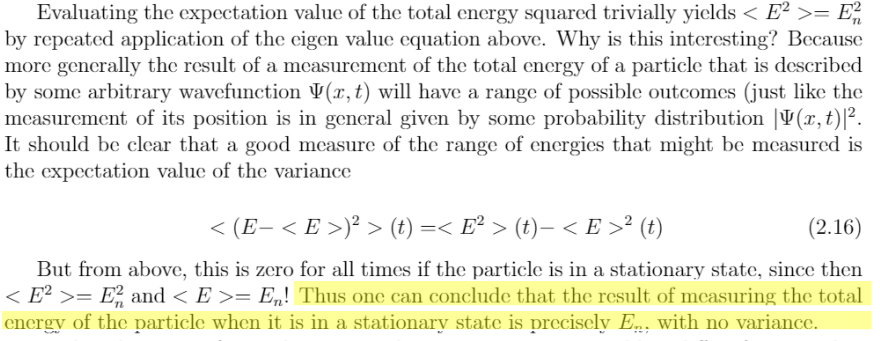
\includegraphics[width = 0.8 \textwidth]{Lecture04/2.png}

\section{Quick note on the de Broglie Wavelength}


From working with the Fourier.jar app from last time, it is clear that there is an inverse relationship between the localization of the wavefunction in position, and the “localization” in the corresponding wavelengths.  This can be quantified better using $\frac{1}{\lambda}$  rather than $\lambda$ to characterize the waves that contribute to a given wavefunction, since mathematically, the Fourier transform of a position dependent function, $f(x), F(k)$, is defined in terms of $k = \frac{2 \pi}{\lambda}$, not $\lambda$. 

$$f(x) = \frac{1}{\sqrt{2 \pi}} \int_{- \infty}^\infty F(k) e^{i k x} dk \Leftrightarrow F(k) = \frac{1}{\sqrt{2 \pi}} \int_{- \infty}^\infty f(x) e^{-i k x} dx$$

From Fourier analysis, $\sigma_{2 \pi / \lambda} \sigma_x > \frac{1}{2}$, or $\sigma_k \sigma_x \geq \frac{1}{2}$, and the equality only holds for Gaussian functions. 

This lies at the heart of the uncertainty principle, as a harmonic wavefunction (one with only one wavelength, completely delocalized in space) has a precisely-defined momentum expectation value: the de Broglie formula relates the momentum to the wavelength $p = \frac{\hbar}{\lambda}$, hence $\sigma_x \sigma_p \geq \frac{\hbar}{2}$. Here, $\sigma_i$ is the standard deviation of the subscripted variable. 
\textit{[showed the .jar demo again and we recognized, quantitatively, this inverse relationship. Whether all in phase or random, the "characteristic length" is inversely proportional to the variance in $k$.]}




\end{document}